 \documentclass{article}
\usepackage[italian]{babel}
\usepackage{hyperref}
\usepackage{graphicx}
\usepackage{xcolor}
\usepackage[sorting=none]{biblatex}
\usepackage[many]{tcolorbox}
\usepackage{float}
\addbibresource{references.bib}

\usepackage{geometry}
\geometry{
 a4paper,
 total={170mm,257mm},
 left=40mm,
 right=40mm,
 top=30mm,
 bottom=40mm,
}
 
\title{Come scrivere una Tesi di Laurea}
\author{Decision \& Control Laboratory\\Politecnico di Bari\\\url{http://dclab.poliba.it}}
\date{\today}

% Colors
\definecolor{dclab_blue}{RGB}{68, 115, 197}
\definecolor{dclab_dark_blue}{RGB}{30, 55, 97}
\definecolor{dclab_light_blue}{RGB}{233, 238, 248}


% Url settings
\urlstyle{tt}
\hypersetup{
    colorlinks=true,
    urlcolor=dclab_blue,
    citecolor=dclab_blue
    % filecolor=magenta,      
    % urlcolor=cyan,
}

% Create a note
\newcounter{nota}
\newtcolorbox[use counter=nota]
  {nota}[1][]
  {title=Nota~\thetcbcounter,
   left=0pt,
   right=0pt,
   fonttitle=\bfseries,
   coltitle=white,
   colframe=dclab_dark_blue,
   colback=dclab_light_blue,
   #1
}   


% Define a custom quote box
\newtcolorbox{customquote}[1][]{
  colback=gray!10, % Light gray background
  colframe=gray!50, % Gray border
  fonttitle=\itshape, % Italic title
  coltitle=black, % Title color
  #1
}

% Other settings
\setlength{\parindent}{10pt} 
\setlength{\parskip}{5pt} 

\usepackage{subcaption}
\usepackage[labelfont=bf, textfont=it, font=small]{caption}
\captionsetup{justification=centering}
\captionsetup{skip=10pt} % Adjust spacing as needed

\usetikzlibrary{shapes, calc, arrows, positioning}
    
\tikzset{
        block/.style = {draw, rectangle,
            minimum height=1cm,
            minimum width=2cm},
        input/.style = {coordinate,node distance=1cm},
        output/.style = {coordinate,node distance=4cm},
        arrow/.style={draw, -latex,node distance=2cm},
        pinstyle/.style = {pin edge={latex-, black,node distance=2cm}},
        sum/.style = {draw, circle, node distance=1cm},
}

\begin{document}

\maketitle

Il titolo ideale per questo documento dovrebbe essere ``\textit{Guida alla Redazione di una Tesi di Laurea presso il Decision \& Control Laboratory (D\&C Lab)}‘’. In questo documento abbiamo raccolto consigli e suggerimenti fondamentali che, a nostro avviso, è indispensabile leggere attentamente prima di iniziare la stesura del vostro elaborato.

\begin{figure}[h]
\centering
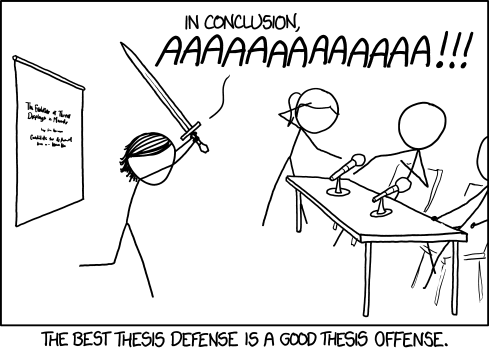
\includegraphics[width=0.5\textwidth]{fig/thesis-defense.png}
\caption{Non si può dire di far parte di una facoltà \href{https://en.wikipedia.org/wiki/Science,_technology,_engineering,_and_mathematics}{STEM} se non si conoscono le vignette di \href{https://xkcd.com/1403/}{xkcd}.}
\label{fig:schema}
\end{figure}

Lo scopo intrinseco di redigere una tesi di laurea consiste nel presentare alla commissione (ma non solo) le proprie capacità e, soprattutto, ciò che si è appreso durante il percorso di studio. La tesi deve dimostrare la capacità di applicare le conoscenze acquisite nel corso del lavoro per risolvere un problema ingegneristico specifico.
Questo documento non si concentra sul tema specifico della vostra tesi, ma sul processo generale di ricerca scientifica necessario per svilupparla. È rivolto sia alle tesi \textit{sperimentali} che a quelle \textit{compilative}, poiché il processo e la struttura del documento sono, nella sostanza, simili.

Prima di addentrarci nella guida, vi consigliamo di leggere \textit{Come si fa una tesi di laurea} \cite{eco2017come} di Umberto Eco, un’opera che ha superato la prova del tempo e che riteniamo di grande valore. Pur essendo piuttosto corposa, speriamo che ne troviate utile il contenuto
Vi suggeriamo inoltre \textit{L’arte della guerra} di Sun Tzu \cite{sun_tzu_arte_della_guerra}, i cui insegnamenti possono rivelarsi preziosi per affrontare al meglio le sfide, sia personali che professionali, come ad esempio la stesura di una tesi di laurea.
\begin{customquote}[title={\textit{Sun Tzu}}]
``Con ordine affronta il disordine, con calma l’irruenza. Questo significa avere il controllo del cuore’’
\end{customquote}
Rimanere calmi e non lasciarsi sopraffare dalla rabbia, affrontare il disordine con ordine, trovare un equilibrio tra il coraggio sconsiderato e la codardia, non affrontare le situazioni senza la dovuta preparazione, essere determinati ma senza ostinazione.

\section{Prima di cominciare}
Prima di cominciare a parlare di come si scrive (o almeno di come ci si prova) una tesi universitaria, è bene chiarire alcuni aspetti burocratici. Durante il percorso universitario ci si ritrova di fronte a una realtà notevolmente diversa da quella della scuola secondaria. La parola d’ordine diventa ``autonomia’', poiché, salvo alcuni vincoli formali, si ha la totale libertà di decidere quando e come sostenere gli esami previsti nel proprio piano di studi.

Anche il percorso di tesi è caratterizzato da tale autonomia. Sebbene l’obiettivo di ogni studente sia la laurea, la strada per raggiungerla può variare notevolmente da un collega all’altro.
\begin{nota}
Pertanto, la responsabilità principale ricade su di voi: dovete essere autonomi nel reperire le informazioni sulle scadenze e sui documenti da consegnare.\end{nota}
\begin{nota}
Ricordate sempre che è buona norma anticipare le procedure, inclusa la firma dei moduli, rispetto alle scadenze stabilite.
\end{nota}

Il nostro ruolo è quello di supportarvi e supervisionare la compilazione dei moduli, ma spetta a voi informarvi in modo proattivo. Per facilitarvi, vi forniamo uno schema riassuntivo dei principali passi necessari. Tuttavia vi chiediamo di studiare attentamente i seguenti link che contengono alcune delle informazioni di cui avete bisogno:
\begin{itemize}
\item \href{http://www.poliba.it/it/procedure-la-laurea}{Procedure per la laurea}
\item \href{http://www.poliba.it/it/tirocini-curriculari}{Tirocini per studenti}
\item \href{https://www.dmmm.poliba.it/index.php/it/tirocini-interni}{Tirocini per studenti (DMMM)}
\item \href{https://www.dmmm.poliba.it/index.php/it/didattica}{Informazioni utili per studenti e laureandi (DMMM)}
\item \href{https://dei.poliba.it/informazioni-per-gli-studenti/}{Informazioni utili per studenti e laureandi (DEI)}
\end{itemize}

\section{Riproducibilità}
L’obiettivo principale da porsi nello sviluppo di una tesi è quello di dettagliare in modo scrupoloso il processo di ricerca adottato. Nel redigere la tesi, la riproducibilità deve essere una priorità costante. Ciò significa che è fondamentale garantire che un collega possa prendere il vostro documento e riprodurre i risultati ottenuti.

Difatti, è di vitale importanza giustificare ogni scelta effettuata durante il percorso. Questo approccio consente di valutare non solo i risultati ottenuti, ma l’intero processo seguito per giungere a tali conclusioni.

\section{Struttura}
La struttura di una tesi può essere varia, ma alcune componenti fondamentali includono sempre un sommario, un’introduzione e le conclusioni. Tra l’introduzione e le conclusioni si collocano i capitoli, ciascuno dei quali è suddiviso in sezioni. Una tesi dovrebbe comprendere almeno due capitoli. Ecco una possibile struttura:
\begin{description}
\item[Sommario:] Una breve sintesi, di solito intorno alle 300 parole, in cui si riassumono la portata, gli obiettivi, i metodi e i risultati della tesi.
\item[Introduzione:] Spiega il contesto della tesi, delineando gli obiettivi del lavoro e descrivendo a grandi linee l’approccio adottato.
\item[Studiodella letteratura:] Riporta le ricerche rilevanti sull’argomento della tesi.
\item[Formulazione del problema e metodo di risoluzione:]  Descrivi dettagliatamente il problema in esame e illustra gli strumenti utilizzati per la sua risoluzione.
\item[Risultati:] Presenta e commenta i risultati ottenuti, spiegandone il significato. Indica risultati attesi e inattesi, fornendo spiegazioni per questi ultimi.
\item[Conclusione:] Riassumi le scoperte chiave e offri possibili sviluppi future basate sui risultati.
\end{description}
Da non dimenticare, inoltre, il frontespizio, l’indice e la bibliografia.

Normalmente, il sommario, l’introduzione e le conclusioni si scrivono \textbf{dopo} aver completato i vari capitoli che compongono la tesi. In alcuni casi, può essere sensato mescolare o separare i capitoli, ma la struttura proposta costituisce un solido punto di partenza.

\section{Scrittura accademica}
La struttura di un testo tecnico/accademico segue un preciso schema:
\begin{description}
\item[Anticipa:] Inizia dicendo ai tuoi lettori ciò che stai per esporre.
\item[Esponi:] Successivamente, trasmetti il messaggio o l’argomento principale.
\item[Riassumi:] Concludi comunicando nuovamente ciò che hai appena illustrato.
\end{description}
Questa struttura è applicabile a vari livelli all’interno di una tesi. A livello complessivo, l’introduzione preannuncia il contenuto, mentre la conclusione sintetizza quanto è stato esposto. I capitoli intermedi costituiscono il nucleo del lavoro. Tuttavia, è fondamentale applicare la medesima logica anche a ogni singolo capitolo, ad esempio, arricchendolo con brevi frasi che introducano il capitolo, in modo da immergere il lettore nella tematica trattata, concludendo poi ogni parte con una sintesi.

Nonostante non esistano regole ferree, l’utilizzo dei simboli matematici è dettato da convenzioni. Molte di queste sono riassunte del \href{https://www.ams.org/publications/authors/AMS-StyleGuide-online.pdf#chapter.149}{Capitolo 12} della guida stilistica dell’American Mathematical Society (AMS).

\section{Studio della letteratura}
Il primo passo di ogni lavoro di tesi che si rispetti è quello di condurre una \textit{review} della letteratura, nota anche come studio della letteratura o stato dell’arte. Questo studio dimostra a chi legge la tesi che l’autore ha una conoscenza approfondita del tema e che quindi può affrontarlo seriamente, proponendo eventualmente soluzioni.

Iniziate identificando gli argomenti chiave della tesi e i termini chiave. Come primo passo, potete avviare una ricerca generale su Google. Successivamente, concentrate la ricerca su lavori scientifici. Sfruttate strumenti come \href{https://scholar.google.com/}{Google Scholar}, \href{https://ieeexplore.ieee.org/Xplore/home.jsp}{IEEE Xplore} e  \href{https://consensus.app/}{Consensus}.

Registrate con precisione tutte le informazioni bibliografiche e categorizzate i contributi dei vari articoli. Per fare questo, potete prendere spunto dal file \href{http://dclab.poliba.it/wp-content/uploads/StudioLetteratura.xlsx}{StudioLetteratura.xlsx} che vi forniamo sul sito del D\&C Lab., in alternativa, sfruttare strumenti di gestione, come \href{https://www.mendeley.com/?interaction_required=true}{Mendeley}, \href{https://www.zotero.org/}{Zotero}, o \href{https://www.jabref.org/}{JabRef}.

La differenza tra una lista di articoli e una \textit{review} della letteratura è che quest’ultima sintetizza le fonti in una panoramica complessa. Nella \textit{review} vanno identificati \textit{trend} e lacune nella letteratura. In una \textit{review} fatta bene  vanno esaminate le metodologie utilizzate negli articoli selezionati e va elaborata una sintesi coerente dei principali risultati e conclusioni. Trovate alcuni trucchi utili in questa presentazione:
\href{https://www.dcu.ie/sites/default/files/students_learning/scientific_lit_review_workshop_ug.pdf}{Scientific Literature Review}.

\section{Ortografia, grammatica e formattazione}
Prestate particolare attenzione alla scrittura, evitando errori grammaticali e ortografici che, purtroppo, sono comuni nelle tesi. Controllate attentamente la formattazione del testo. Un testo disordinato o sciatto può lasciare una pessima impressione. Assicuratevi che il vostro lavoro sia presentato in modo professionale e coerente.

Utilizzate un nuovo paragrafo quando cambiate argomento, evitando di andare a capo ogni volta che inserite un punto. Preferite frasi brevi. Se notate frasi troppo lunghe, rileggetele attentamente e spezzatele in modo che siano più facili da comprendere.

Usate maiuscole con parsimonia, limitandole ai contesti essenziali. Evitate sottolineature e grassetto, riservate il corsivo ai termini stranieri e a quelli che desiderate enfatizzare. Evitate punti esclamativi e puntini sospensivi, e riducete al minimo l’uso di elenchi puntati e numerati per mantenere la chiarezza.

Vi preghiamo di non apportare modifiche ai margini né alla dimensione del carattere. Il \textit{template} fornito soddisfa tutte le richieste del dipartimento.

\section{Citazioni, fonti online e intelligenza artificiale}
Le citazioni consistono nell’atto di riportare contenuti tratti da opere di altri autori. È un dovere intellettuale citare chiaramente le fonti all’interno del proprio testo, sia per onestà intellettuale sia per distinguere adeguatamente il contributo originale da ciò che è tratto dal pensiero altrui.

\begin{nota} Non si può utilizzare il materiale di qualcun altro senza citazione e riferimento. \end{nota}

In passato, l’assenza di strumenti per rilevare il plagio rendeva più facile che l’illecito passasse inosservato. Tuttavia, con l’uso diffuso di software per il rilevamento del plagio, i casi di plagio sono ora più facili da individuare. È necessario citare tutte le fonti utilizzate nel corso dell’analisi per consentire a chiunque di riprodurre il vostro lavoro. Quando riprendete integralmente le frasi di un autore, inseritele tra virgolette e citate la pagina dell’opera da cui sono tratte.

La vastità di informazioni disponibili su Internet può rappresentare una risorsa preziosa, ma è essenziale adottare un approccio critico nella selezione e nell’utilizzo di tali contenuti. Internet è spesso sfruttato come un modo facile per riempire le pagine di una tesi.

Gli strumenti di intelligenza artificiale generativa, inclusi gli LLM (Large Language Models), possono supportare il lavoro di tesi, ma non devono sostituire il contributo personale e la comprensione critica dello studente. L’uso di testi generati da LLM è ormai un’area grigia dal punto di vista etico. Presentare il lavoro di qualcun altro come proprio è considerato plagio, ma quando si tratta di testi generati dall’intelligenza artificiale, non è chiaro dove finisca il contributo individuale e inizi il plagio. Per definizione, gli LLM prendono testi umani e li ``codificano’’ per un uso successivo come modello statistico. Il risultato degli LLM potrebbe quindi corrispondere a testi già presenti su Internet. Pertanto, gli LLM possono generare plagio. Inoltre, gli LLM possono generare dichiarazioni false o inesatte. Il modello può generare informazioni correttamente formattate, come riferimenti, che in realtà non esistono.

\begin{nota}
Lo studente, in qualità di autore unico della tesi, è responsabile di tutti i contenuti della tesi. Non è accettabile inserire testi, codice, formule o risultati che non siano stati compresi e verificati.
\end{nota}

La valutazione del lavoro di tesi riguarda la qualità del ,lavoro, ma soprattutto la comprensione dei contenuti e il contributo personale dello studente. Questi aspetti saranno discussi durante le revisioni intermedie e nella preparazione della discussione finale. Un elaborato essenziale, accurato e pienamente padroneggiato è preferibile a un testo esteso che lo studente non sappia spiegare. Preferiamo leggere e correggere una tesi di 10 pagine scritta da un umano, piuttosto che 100 pagine generate da ChatGPT. Fate poco ma fatelo bene.

Gli strumenti di correzione grammaticale basati sull'intelligenza artificiale hanno compiuto notevoli progressi nel corso del tempo. L’uso di questi strumenti è diverso rispetto alla generazione di testi tramite prompt degli LLM. Questi strumenti utilizzano testi scritti da esseri umani come base per apportare modifiche e suggerimenti. Questo processo è simile a chiedere a un amico o a un collega di rivedere un testo e di proporre suggerimenti. Di conseguenza, l’utilizzo di strumenti AI con testi prescritti non solleva preoccupazioni etiche, come il plagio, ed è generalmente accettato.

\section{Didascalie delle figure}
Le didascalie delle figure svolgono un ruolo cruciale nella presentazione visiva della vostra tesi. Non dovrebbero limitarsi a brevi descrizioni come ``Distribuzione di X’', ma piuttosto svolgere un ruolo informativo. Ogni didascalia dovrebbe, almeno, offrire una descrizione dettagliata di ciò che è visibile nella figura, e possibilmente, indicare al lettore cosa osservare e apprendere dalla stessa. È accettabile che vi sia una certa sovrapposizione concettuale tra le didascalie e il testo principale. Tuttavia, evitate duplicazioni e cercate di offrire nuove informazioni nella didascalia.

\section{Prendi appunti}
Lo scopo della tesi è condurre una ricerca su un argomento, esplorare la letteratura, affrontare il problema da diverse angolazioni e acquisire una comprensione approfondita. Tutto ciò implica che prendere appunti è essenziale! Scrivere una tesi richiede mesi di lavoro, e non è possibile ricordare i dettagli dei metodi utilizzati nei primi giorni di ricerca. All’inizio non è necessario scrivere un testo dettagliato, poiché non sapete ancora cosa sia davvero importante. Limitatevi a annotare le scoperte rilevanti e le impostazioni dei parametri.

Non esiste una regola che imponga di scrivere l’intera tesi in un’unica sessione non stop, in cui non dormite per tre settimane. Non cercate di essere perfezionisti! La tesi verrà scritta in diverse fasi, e ogni parte potrà essere perfezionata in seguito. Non cercare di fare tutto perfetto fin da subito. Se tentate di farlo, rischiate di scoraggiarvi quando, inevitabilmente, ciò che scrivete non sarà perfetto. Scrivete alcune idee e occupatevi di migliorarle durante lo sprint finale.

La scrittura di una tesi non segue un processo lineare. Non si scrive prima il capitolo 1, poi il 2, e infine il 3. Scrivere una tesi è più simile al controllo di un sistema in retroazione. Iniziate con l’introduzione, passate al modello matematico e poi alle simulazioni. Successivamente, riceverete feedback sia da voi stessi sia dai vostri tutor e riscriverete le sezioni che necessitano di miglioramenti. Questo ciclo continua fino a raggiungere un equilibrio, seguendo un approccio di sviluppo a spirale, tipico nella gestione dei progetti \cite{boehm1998using}.
\begin{figure}[H]
\begin{center}
\begin{tikzpicture}[auto]
\node [input, name=input, label=left:$u(t)$] {};
\node [sum, right=of input] (sum) {};
\node [coordinate, right=of sum, label=above:$x(t)$] (xl) {};
\node [block, right=of xl] (controller) {$G(s)$};
\node [coordinate, right=of controller] (swi) {};
\node [output, right=2cm of swi, label=right:$y(t)$] (output) {};
\node [block, below= of controller] (feedback) {$H(s)$};
\draw [draw,->] (input) -- node[pos=0.9, above] {$+$} (sum);
\draw [->] (sum) -- (controller);
\draw [->] (controller) -- (output);
\draw [->] (swi) |- (feedback) ;
\draw [->] (feedback) -| node[pos=0.95, right] {$-$} (sum);
\end{tikzpicture}
\end{center}
\caption{Diagramma a blocchi di un tipico sistema di controllo.}
\label{fig:control-system}
\end{figure}

\section{\LaTeX{} e BibTeX}
Come forse abbiamo già accennato, la vostra tesi sarà redatta in \LaTeX{} e non in MS Word. Questo non è un capriccio, ma scelta consapevole basata su vantaggi significativi. \LaTeX{} funziona in modo eccellente per documenti di grandi dimensioni, soprattutto quando arricchiti da numerose figure ed equazioni. Oltre a garantire stabilità, \LaTeX{} ti assiste nella strutturazione del lavoro, nella gestione dei riferimenti incrociati e delle citazioni, offrendo una composizione tipografica di qualità professionale.

Durante la stesura della tesi, dovrai leggere e organizzare un'ampia mole di articoli scientifici. BibTeX è lo strumento che \LaTeX{} utilizza per gestire i riferimenti bibliografici. Pur potendo sembrare inizialmente complesso, BibTeX offre un modo efficiente per gestire i riferimenti senza dover digitare manualmente ciascuno di essi con la corretta formattazione. Ti consigliamo di cercare le voci BibTeX per gli articoli che hai letto, ottenendole tramite \href{https://scholar.google.com/}{Google Scholar}, e di aggiungerle al tuo file \texttt{.bib}, mediante la procedura indicata in questo video:
\href{https://www.youtube.com/watch?v=hwTpPW6N9og}{How to Use Reference, Citation and BibTex in LaTex, Overleaf, ShareLatex}
\begin{figure}
\centering
\subfloat[Da \href{https://xkcd.com/1301/}{xfcd: File Extension}]{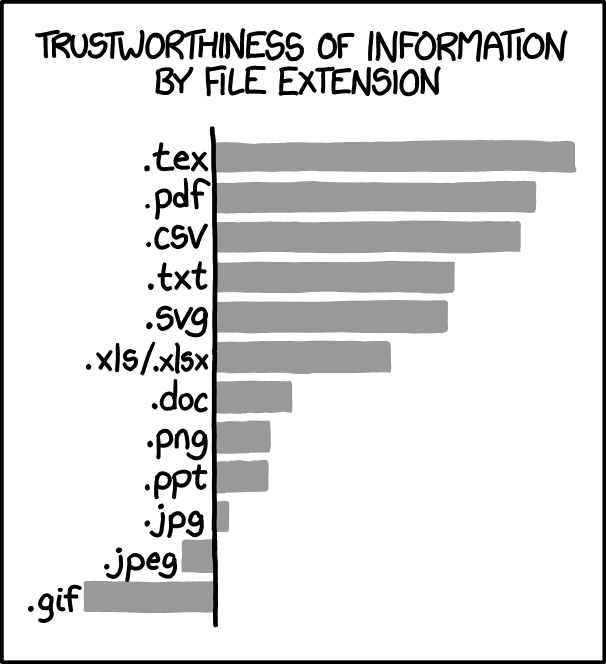
\includegraphics[width=0.4\textwidth]{fig/file_extensions_2x.png}}
\hfill
\subfloat[Da \href{https://www.pinteric.com/miktex.html}{Marko Pinteric}]{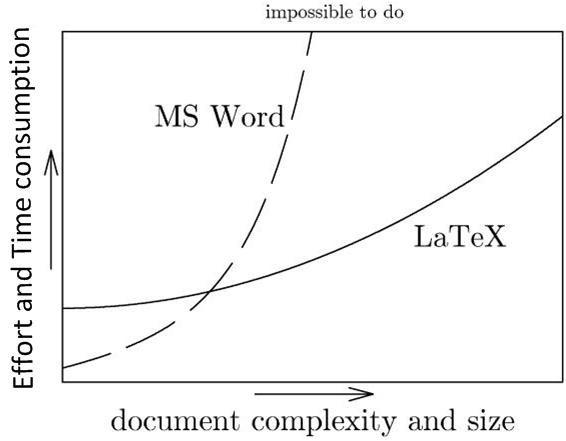
\includegraphics[width=0.55\textwidth]{fig/latex_word.jpg}}
\label{fig:file_extensions_2x}
\caption{ddd}
\end{figure}
Per semplificare il passaggio a \LaTeX{}, vi consigliamo di utilizzare un editor online gratuito, \href{https://it.overleaf.com}{Overleaf}, che non richiede installazione. Abbiamo preparato due template per facilitarvi nella stesura della tesi e della relazione di tirocinio, scaricabili dai seguenti link:
\begin{itemize}
\item \href{https://decision-and-control-lab.github.io/dclab-template/templates/}{Template Decision Control}
\end{itemize}

Per utilizzare i \textit{template} dovrete creare un account su Overleaf oppure provvedere a installare una distribuzione locale di LateX.

Vi consigliamo di non cancellare gli esempi presenti nel template; al contrario, utilizzateli per comprenderne il funzionamento. Non apportare modifiche ai margini e alla grandezza del carattere. \textbf{Il template fornito rispetta tutte le richieste del dipartimento.} Troverete ulteriori risorse utili nei seguenti link, sebbene non siano strettamente necessari grazie al template che vi abbiamo inviato:
\begin{itemize}
\item \href{http://www.guitex.org/home/images/doc/GuideGuIT/IntroTesi.pdf}{Scrivere una tesi di laurea in LaTeX}
\item \href{https://mathspp.com/blog/write-your-thesis-in-latex}{Write your thesis in LaTeX}
\item \href{https://joaoramiro.medium.com/10-tips-on-writing-a-master-thesis-in-latex-with-overleaf-7376e07aad20}{10 tips on writing a master thesis in latex with overleaf}
\end{itemize}

\printbibliography

\end{document}
